%%%%%%%%%%%%%%%%%%%%%%%%%%%%%%%%%%%%%%%%%
% Beamer Presentation
% LaTeX Template
% Version 1.0 (10/11/12)
%
% This template has been downloaded from:
% http://www.LaTeXTemplates.com
%
% License:
% CC BY-NC-SA 3.0 (http://creativecommons.org/licenses/by-nc-sa/3.0/)
%
%%%%%%%%%%%%%%%%%%%%%%%%%%%%%%%%%%%%%%%%%

 
%----------------------------------------------------------------------------------------
%	PACKAGES AND THEMES
%----------------------------------------------------------------------------------------

\documentclass[15pt]{beamer}
\usepackage[utf8]{inputenc}
\usepackage{amsmath}
\usepackage{graphicx}
\usepackage{hyperref}
\usepackage{float}
\usepackage{wrapfig}
\usepackage{comment} % enables the use of multi-line comments (\ifx \fi) 
\usepackage{lipsum} %This package just generates Lorem Ipsum filler text.
%\usepackage[french]{babel}
\pdfmapfile{+sansmathaccent.map}

\mode<presentation> {

% The Beamer class comes with a number of default slide themes
% which change the colors and layouts of slides. Below this is a list
% of all the themes, uncomment each in turn to see what they look like.

%\usetheme{default}
%\usetheme{AnnArbor}
%\usetheme{Antibes}
%\usetheme{Bergen}
%\usetheme{Berkeley}
%\usetheme{Berlin}
%\usetheme{Boadilla}
%\usetheme{CambridgeUS}
%\usetheme{Copenhagen}
%\usetheme{Darmstadt}
%\usetheme{Dresden}
%\usetheme{Frankfurt}
%\usetheme{Goettingen}
%\usetheme{Hannover}
%\usetheme{Ilmenau}
%\usetheme{JuanLesPins}
%\usetheme{Luebeck}
\usetheme{Madrid}
%\usetheme{Malmoe}
%\usetheme{Marburg}
%\usetheme{Montpellier}
%\usetheme{PaloAlto}
%\usetheme{Pittsburgh}
%\usetheme{Rochester}
%\usetheme{Singapore}
%\usetheme{Szeged}
%\usetheme{Warsaw}

% As well as themes, the Beamer class has a number of color themes
% for any slide theme. Uncomment each of these in turn to see how it
% changes the colors of your current slide theme.

%\usecolortheme{albatross}
\usecolortheme{beaver}
%\usecolortheme{beetle}
%\usecolortheme{crane}
%\usecolortheme{dolphin}
%\usecolortheme{dove}
%\usecolortheme{fly}
%\usecolortheme{lily}
%\usecolortheme{orchid}
%\usecolortheme{rose}
%\usecolortheme{seagull}
%\usecolortheme{seahorse}
%\usecolortheme{whale}
%\usecolortheme{wolverine}

%\setbeamertemplate{footline} % To remove the footer line in all slides uncomment this line
\setbeamertemplate{footline}[page number] % To replace the footer line in all slides with a simple slide count uncomment this line

%\setbeamertemplate{navigation symbols}{} % To remove the navigation symbols from the bottom of all slides uncomment this line
}

\usepackage{graphicx} % Allows including images
\usepackage{booktabs} % Allows the use of \toprule, \midrule and \bottomrule in tables

%----------------------------------------------------------------------------------------
%	TITLE PAGE
%----------------------------------------------------------------------------------------

\title{Multilayer stream graphs} % The short title appears at the bottom of every slide, the full title is only on the title page
\subtitle{JFLI Workshop - 2019}
\author{Pimprenelle Parmentier \\ M1 student\\ Riken AIP} % Your name

%\logo{} 
\institute{\textit{pimprenelle.parmentier@polytechnique.edu}} 
\date{} 
\subject{JFLI Workshop - 2019}



\begin{document}

\begin{frame}
\titlepage % Print the title page as the first slide
\centering
\textbf{Supervisors :} \\
Tiphaine Viard {\footnotesize(Riken AIP)}\\
Benjamin Renoust {\scriptsize(Institute for Datability Science}, {\footnotesize Osaka University)}\\
Jean-François Baffier {\scriptsize(Japan Society for the Promotion of Science},{\footnotesize Tokyo Institute of Technology)}
\end{frame}

%\begin{frame}
%\frametitle{Plan} % Table of contents slide, comment this block out to remove it
%\tableofcontents % Throughout your presentation, if you choose to use \section{} and \subsection{} commands, these will automatically be printed on this slide as an overview of your presentation
%\end{frame}

%----------------------------------------------------------------------------------------
%	PRESENTATION SLIDES
%----------------------------------------------------------------------------------------

%------------------------------------------------
\begin{frame}{Introduction}
\textbf{Graphs} : interactions (edges) between individuals (nodes).
\[
	G=(V,E)
\]
\pause
\begin{minipage}{0.4\linewidth}
{\large A few examples :}
\begin{itemize}
    \item social interactions
    \item biological interactions
    \item IP network
    \item transportation network
\end{itemize}
\end{minipage}
\pause
\begin{minipage}{0.5\linewidth}
\begin{figure}
	\centering
    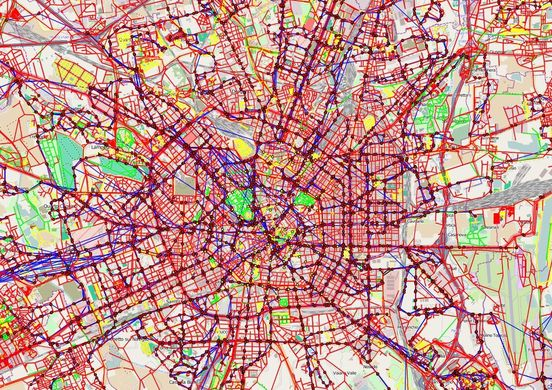
\includegraphics[width=\textwidth]{img/multimodalTransport.jpg}
    \label{fig:exmultitransport}
\end{figure}
\end{minipage}
\pause

$\Rightarrow$ {\large More complex systems : How to deal with...}
\begin{itemize}
    \item time-dependence ?
    \item different types of nodes and/or different types of links ?
\end{itemize}
\end{frame}

\begin{frame}{Multilayer graphs : complex structures}

\[
	M=(V_M,E_M,V,L)
\]
\begin{minipage}{0.4\textwidth}
\begin{footnotesize}
$V = (MAP,MB,YYA)$\\
$L = $(conferences, relationship types)\\
$V_M = $((MAP/ECCS'13/Talk to each other), etc )\\
$E_M = $Edges between elements of $V_M$
\end{footnotesize}
\end{minipage}
\begin{minipage}[r]{0.59\textwidth}
\begin{figure}
    \flushright
    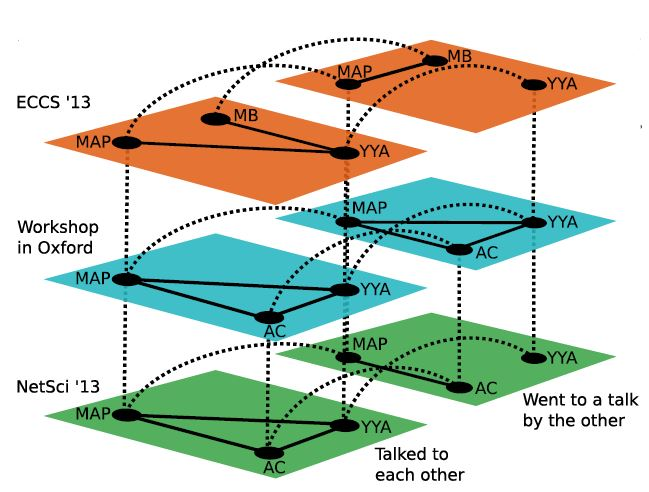
\includegraphics[width=0.8\textwidth]{img/exMulti.jpg}
    \label{fig:exmultitransport}
\end{figure}
\end{minipage}
$$
\left.
\begin{array}{l}
    \text{ Different types of interaction}\\
    \text{ Different types of nodes}
\end{array}
\right \}\rightarrow \textbf{More complex structures}
$$

\end{frame}





\begin{frame}{Stream Graphs : time-dependance}

\[
	S=(T,V,W,E)
\]
\medskip

\begin{minipage}{0.4\textwidth}
\begin{footnotesize}
$T=[0,10]$\\
$V=(a,b,c,d)$\\
$W = ((t,u) | u \text{ appears at } t)$\\
$E = ((t,(u,v)) | (u,v) \text{ appears at } t)$
\end{footnotesize}
\end{minipage}
\begin{minipage}[r]{0.55\textwidth}
\begin{figure}
    \flushright
    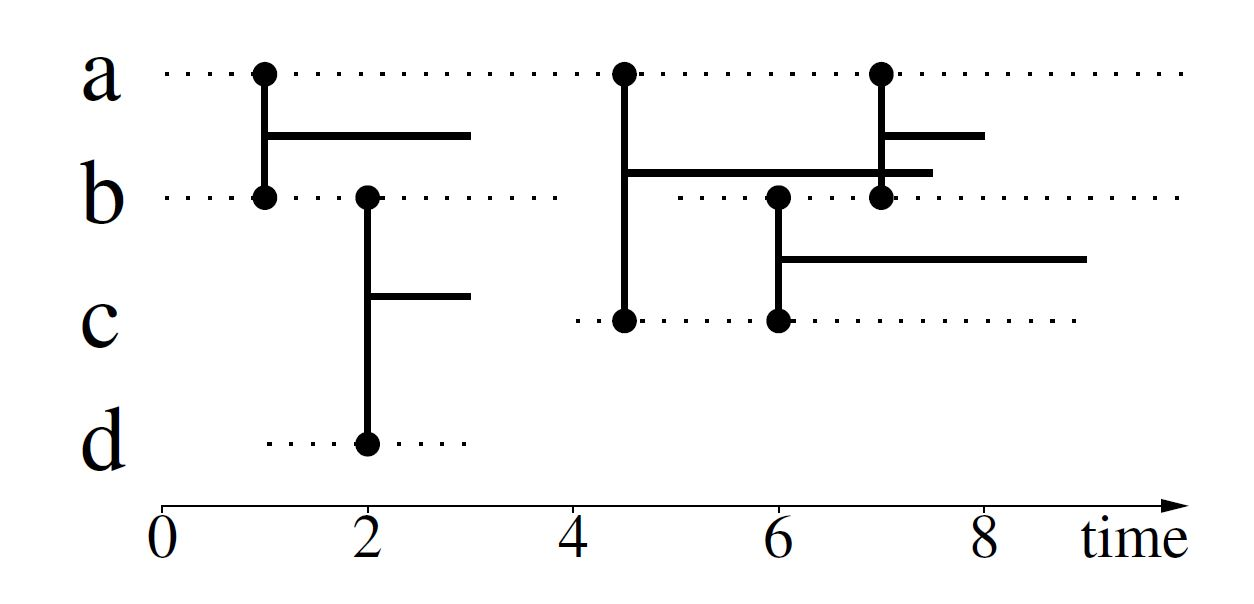
\includegraphics[width=0.8\textwidth]{img/exampleStream.JPG}
    \label{fig:exstream}
\end{figure}
\end{minipage}
\medskip

\begin{itemize}
    \item nodes can appear or desappear in function of continuous time
    \item links can appear or desappear in function of continuous time
\end{itemize}
\smallskip
\centering
$\rightarrow \textbf{Model interactions over time}$





\end{frame}

\begin{frame}{The multilayer stream graph}
\[
G=(T,T_M,V,W_M,E_M,\cal{L})
\]

\begin{figure}
    \centering
    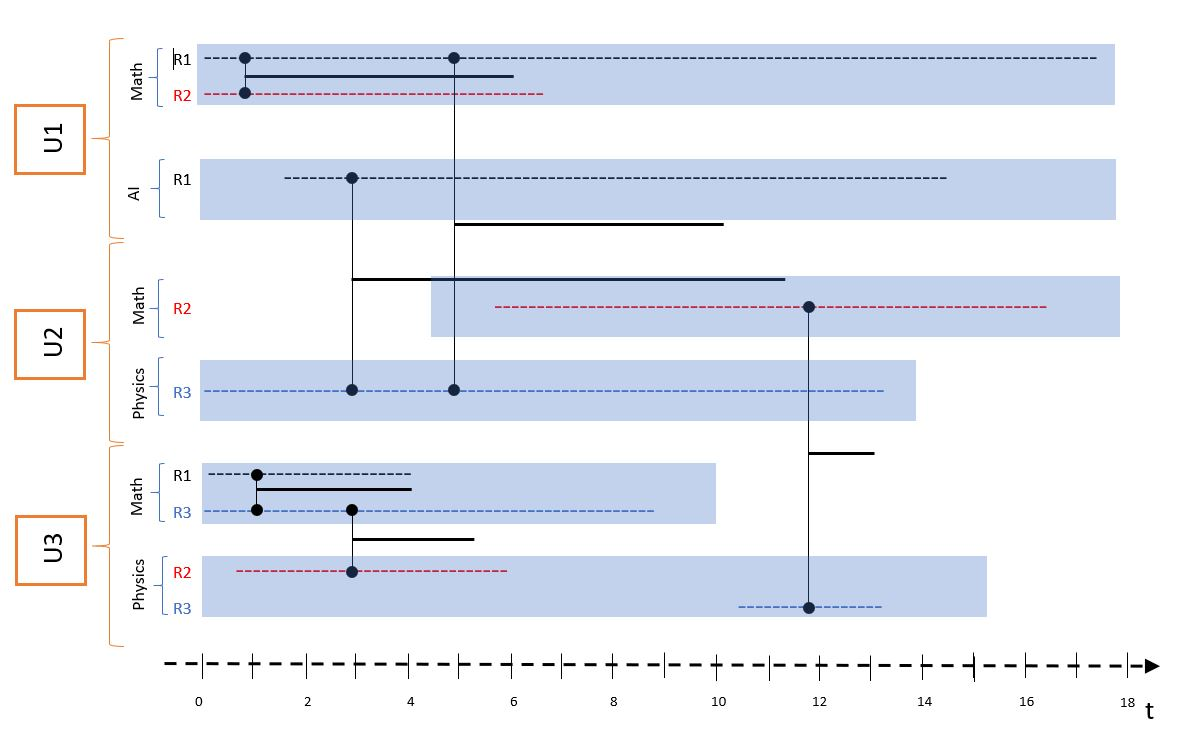
\includegraphics[width=\linewidth]{img/chercheurs.jpg}
    \label{fig:chercheurs}
\end{figure}
\end{frame}

\begin{frame}{The multilayer stream graph}
\[
G=(T,T_M,V,W_M,E_M,\cal{L})
\]
\begin{minipage}{0.69\linewidth}
\begin{figure}
    \centering
    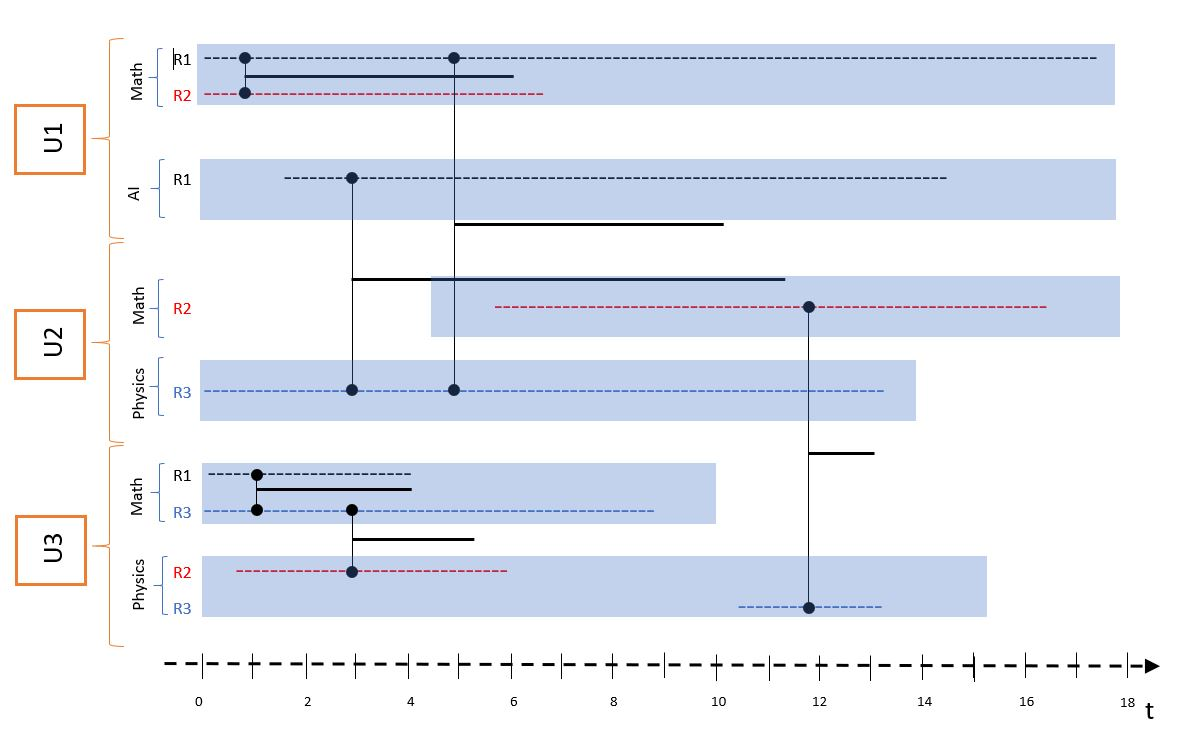
\includegraphics[width=\linewidth]{img/chercheurs.jpg}
    \label{fig:chercheurs}
\end{figure}
\end{minipage}
\begin{minipage}{0.3\textwidth}
\begin{footnotesize}
$T=[0,18]$\\
${\cal L} = (Uni,Dept)$\\
$V=(R1,R2,R3)$\\
\end{footnotesize}
\end{minipage}


$W_M = ((t,(R1,U1,Math))| t \in [0,18]), etc)$\\
$E_M= ((t,(R1,U1,Math),(R2,U2,Math)| t \in [1,6]), etc)$\\
$T_M= (([0,10],(U3,Math)),etc)$
\end{frame}

\begin{frame}{Possibilities}
Find the "decisive" times and and nodes/links/layer : stop a diffusion, find a weakness in the network...

\begin{figure}
	\centering
    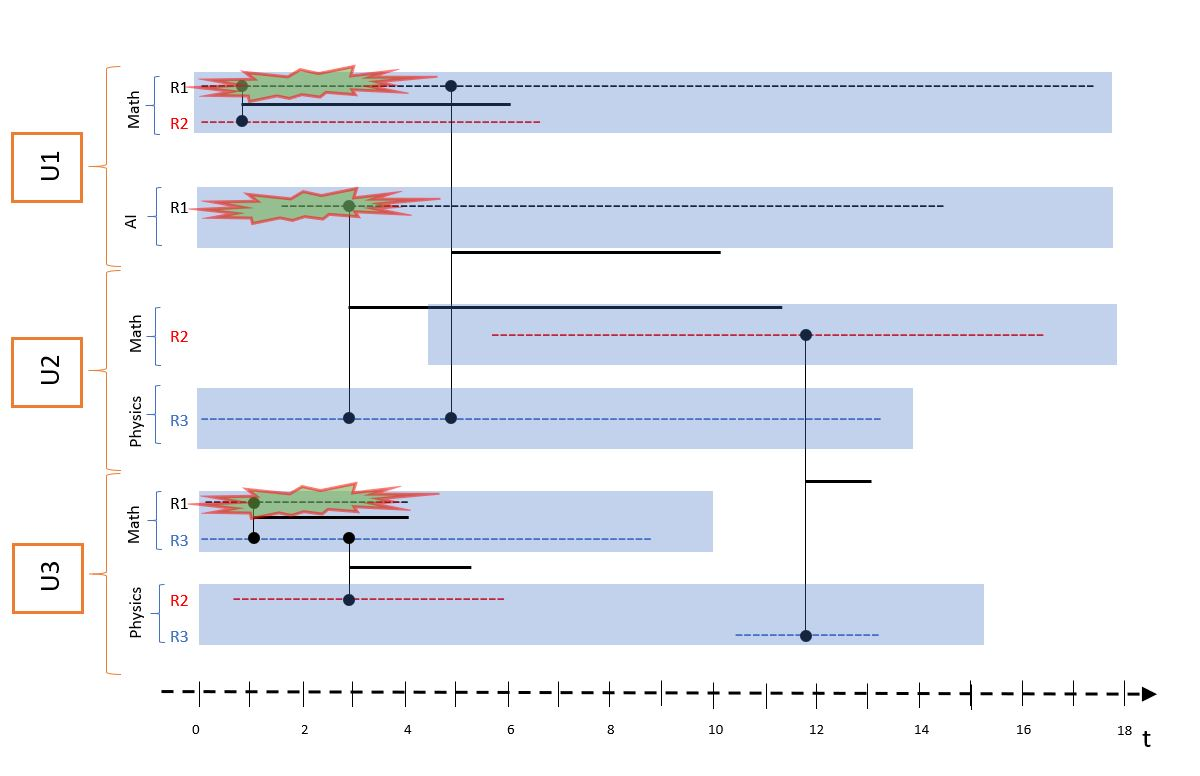
\includegraphics[width=\linewidth]{img/epidemiet0.jpg}
    \label{fig:chercheurs}	
\end{figure}
\end{frame}
\begin{frame}{Possibilities}
Find the "decisive" times and and nodes/links/layer : stop a diffusion, find a weakness in the network...
\begin{figure}
	\centering
    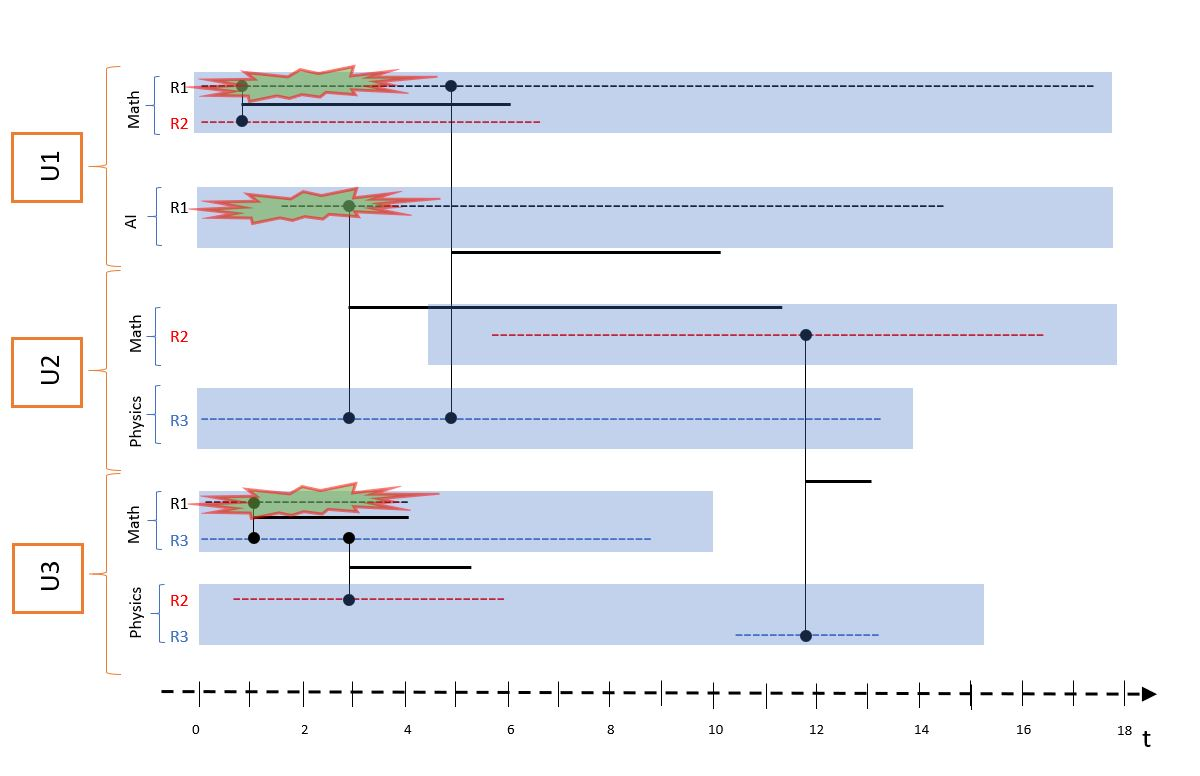
\includegraphics[width=\linewidth]{img/epidemiet0.jpg}
    \label{fig:chercheurs}	
\end{figure}
\end{frame}

\begin{frame}{Possibilities}
Find the "decisive" times and and nodes/links/layer : stop a diffusion, find a weakness in the network...
\begin{figure}
	\centering
    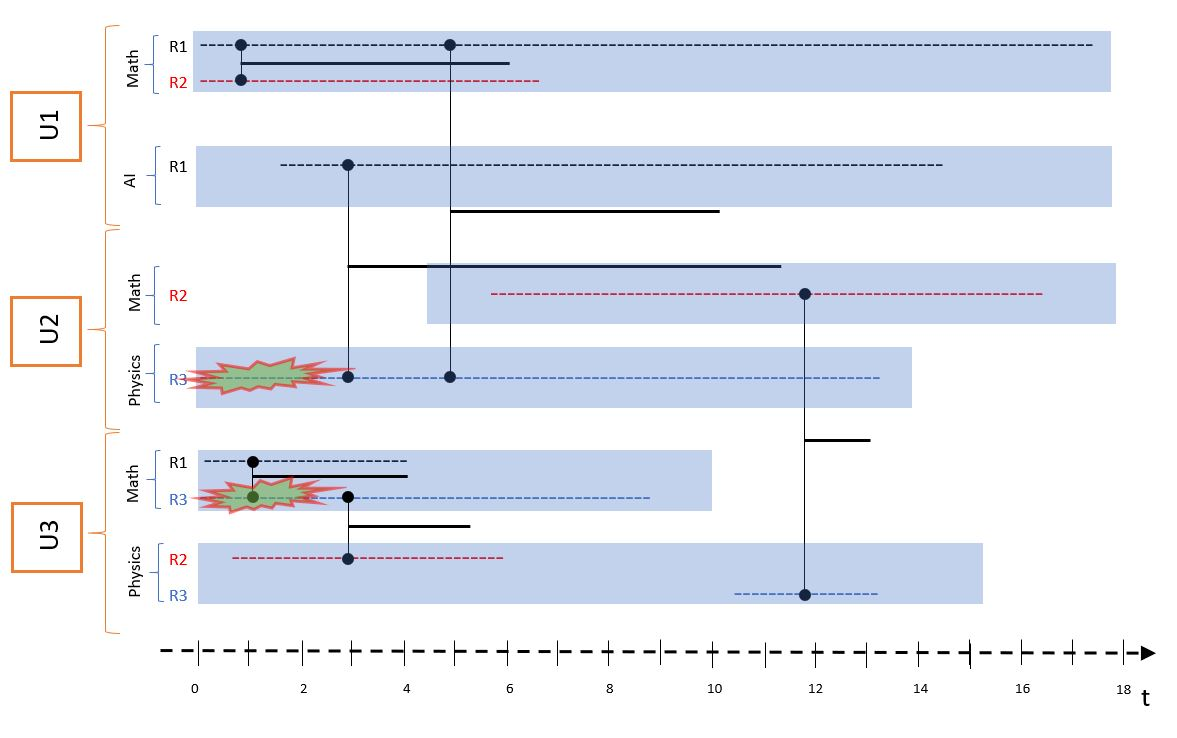
\includegraphics[width=\linewidth]{img/epidemiet1.jpg}
    \label{fig:chercheurs}	
\end{figure}
\end{frame}

\begin{frame}{Possibilities}
Measure "influence" : find a "precursor", find which parameter are "important" and which are not (ex : most of researchers in dept D in university U at time T became "influent") ...\pause
\end{frame}
\begin{frame}{Possibilities}
     measure "intrication" : how much a group of layers are "superimposed" (ex: the relationships of type "co-workers in this company" are "strongly correlated" to most of the overall relationships)\pause
\end{frame}
\begin{frame}{Possibilities}
     determinate if two multilayer-streams have the same structure (isomorphism)
\end{frame}

\begin{frame}{Thank you !}

Resume :
\[
G=(T,T_M,V,W_M,E_M,\cal{L})
\]
\begin{itemize}
	\item Complex structures (different layers of nodes) which change with time...
	\item What we have done : formal object, computational object 
	\item Many possibilities for the future...
\end{itemize}



\end{frame}
\end{document}